\documentclass[12pt,fleqn]{article}\usepackage{../../common}
\begin{document}
Ders 1-15

Makaskirişler (Truss)

Bir makaşkırış esneyebilen çubuklardan (bar) oluşur, bu çubular birbirine
bağlantı pimleri (pin joint) ile bağlıdır. Bağlantı pimi derken şunu
kastediyorum, çubukları esnetmek özellikle uzunluğu yönünde kuvvet gerektirir,
ama pim etrafında çubukları döndürmek efor gerektirmez.

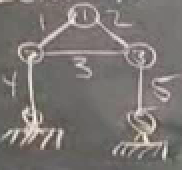
\includegraphics[width=10em]{compscieng_1_15_01.png}

Mesela resimdeki 3 no'lu çubuğu sağa ve sola esnetmek zor, ama o çubuğu
3 no'lu pim etrafında döndürmek kolay.

Bu derste iki boyutlu makaşkırişler incelenecek, daha önce iki boyutlu yay-kütle
sistemini incelediğimiz gibi; muhakkak üç boyutlu makaşkırış sistemleri de var
ama iki boyut üzerinde ana başlıkları daha rahat olarak inceleyebiliriz.













[devam edecek]

\end{document}
